%\documentclass[a4paper,10pt]{jarticle}
%\documentclass[]{jarticle}
\documentclass[10pt]{jarticle}

%\usepackage{graphicx}
\usepackage[dvipdfmx]{graphicx}
\usepackage{eclbkbox} %breakbox用

%本文領域を広め(空白箇所マージン領域を小さめ)に設定
\setlength{\textwidth}{179mm}
\setlength{\textheight}{251mm}
\setlength{\topmargin}{-2cm}
\setlength{\oddsidemargin}{-1cm}
\setlength{\evensidemargin}{-1cm}

\begin{document}

\title{情報工学実験IIレポート(探索アルゴリズム2)}
\author{曜日&グループ番号: 月&グループ0} %
\date{2011年12月23日}

\maketitle

\begin{abstract}
このレポート(ファイル)は、「情報工学実験II・探索アルゴリズムその
2\cite{info2-search2}」の実験レポートの骨組みを例示している。
あくまでも例示であって、全てをこの通りに従う必要はないが、
指示された項目を含めた上で、
報告書として他者が読みやすいレポートとなるように工夫する事。
\end{abstract}

\section*{グループメンバ}
(補足:レベル毎に \underline{全員が協力して実施} した上で、レベル毎にレポートをまとめる担当者を決め、全体を一つのレポートとして整理すること。)
\begin{itemize}
 \item 945734J 當間愛晃: 担当Level1.1, 1.2, 3.4
 \item 945700 hoge: 担当Level2.1, 2,2, 3.5
 \item 945700 hoge: 担当Level3.1, 3.3
 \item 945700 hoge: 担当Level3.2
\end{itemize}

\section*{提出したレポート一式について}
レポート一式は
\verb|``naha:/home/home/teacher/tnal/jikken1-fri/e945734/''|
にアップロードした。
提出したファイルのディレクトリ構成は以下の通りである。\\
(補足:必ず下記のように整理しろという指定ではない。
自分たちでやりやすいようにLevel毎に整理しても構わない)
\begin{breakbox}
\begin{verbatim}
./src/      # 作成したプログラム一式
./report/   # レポート関係ファイル.図ファイルを含む.
\end{verbatim}
\end{breakbox}

\newpage

\section{Level1: 線形分離可能なOR問題への適用}
\subsection{課題説明}
2入力1出力で構成される単純パーセプトロン(ニューラルネットワーク)を
用いて、
4つの教師信号を用意したOR問題へ適用し、
重みが適切に学習可能であることを確認する。
また、学習が収束する様子をグラフとして示す。

 %課題説明
\subsection{OR問題を学習させた際の誤差収束度合いについて}
\subsubsection{実験結果}
NNでは重みを更新する毎に誤差が減るように学習を行うが、
その学習の様子は初期の重みをどのように設定したか、
学習に用いたパラメータをどのように設定したか、
といった対象問題以外の要素に影響して学習の様子が変化する。
シード値を変えた際の学習収束回数を表\ref{table:level1}に示す。
シード値を10回変更して学習させた際の重みを更新する様子を図
\ref{fig:level1-1}に、
その平均をプロットした平均推移値を図\ref{fig:level1-2}に示す。
なお、平均値を求める際には10回分の実行データを加工して統合,平均値を算出した。
具体的には一行ごとに実行データから抜き取り,10回分を加算し,加算回数で割って求めている。
(src/bp\_mo配下のintegration.shを参照)

\begin{table}[htb]
 \begin{center}
  \caption{OR問題の学習に要した回数}
  \label{table:level1}
  \begin{tabular}[htb]{r|l} \hline
   シード値 & 収束した回数 \\ \hline \hline
   1000 & 96 \\ \hline
   2000 & 90 \\ \hline
   3000 & 111 \\ \hline
   4000 & 109 \\ \hline
   5000 & 93 \\ \hline
   6000 & 99 \\ \hline
   7000 & 100 \\ \hline
   8000 & 114 \\ \hline
   9000 & 113 \\ \hline
   10000 & 94 \\ \hline \hline
   10試行の平均値 & 101.9 \\ \hline
  \end{tabular}
 \end{center}
\end{table}


\begin{figure}[h]
 \begin{center}
  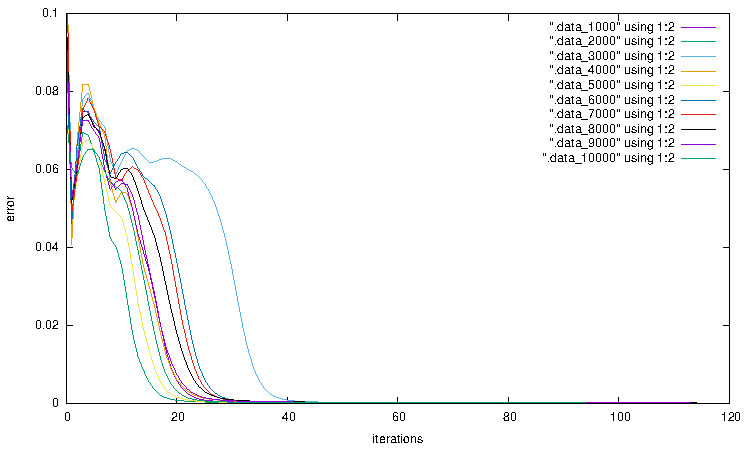
\includegraphics[width=10.0cm]{figs/level1/iterations_vs_error.pdf}
  \caption{重みを更新する様子}
  \label{fig:level1-1}
 \end{center}
\end{figure}

\begin{figure}[h]
 \begin{center}
  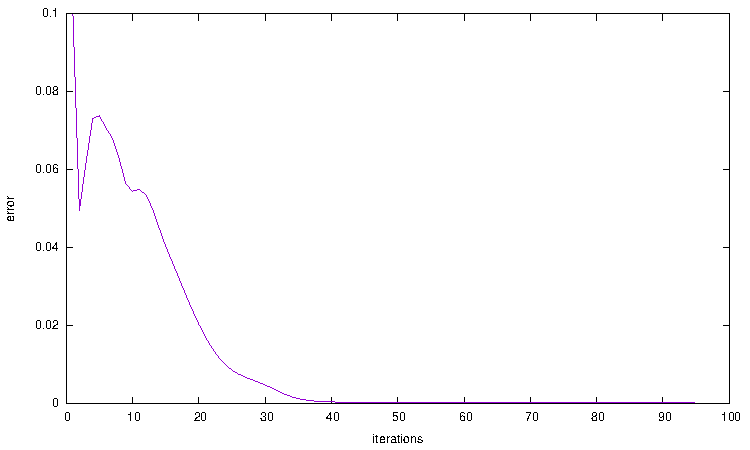
\includegraphics[width=10.0cm]{figs/level1/ave.pdf}
  \caption{重みを更新する様子(平均値)}
  \label{fig:level1-2}
 \end{center}
\end{figure}


\subsubsection{考察}
実験よりわかったことを以下に箇条書きする.\\
\begin{itemize}
	\item すべてFINISH2で終わったため,誤差が最小誤差より小さくなっている.
	\item 実験が収束したのは100前後で,seed値をこれ以上大きくしてみても同じように100前後で収束すると推測する.
	\item 学習曲線は,errorが0.05くらいまで急激に下がり,その後若干上がり,そのあと最小誤差へと遷移している.
\end{itemize}




\newpage

\section{Level2: 線形分離不可能なExOR問題への適用}
\subsection{$B2]Bj@bL@(B}
3$B<oN`$NO"B34X?t(B$y=x^2$$B!"(B$z=x^2+y^2$$B!"(B$y=-x \times cos(x)$$B$K$D$$$F!"(B
$B:G5^9_2<K!$NE,MQ$rDL$7$FC5:w5sF0$r4Q;!$7$?!#(B
$B0J2<$G$O$^$:6&DLItJ,$G$"$k:G5^9_2<K!$NC5:w<jB3$-$K$D$$$F!"(B
$B%U%m!<%A%c!<%H$rMQ$$$F2r@b$9$k!#(B
$B$=$N8e!"(B3$B<oN`$N4X?tKh$K%W%m%0%i%`$NJQ992U=j!"(B
$B4Q;!0U?^4Q;!J}K!!"4Q;!7k2L!"9M;!$K$D$$$F@bL@$9$k!#(B


\subsection{Level 2$B6&DLItJ,(B}
$B!JJdB-!'(BLevel2.1, 2.2, 2.3 $B$K$O6&DL$9$kItJ,$,B?$$$?$a!"(B
$B6&DLItJ,$OFHN)$7$FJs9p$9$k$HNI$$$G$7$g$&!K(B

\subsubsection{$BC5:w$N<jB3$-!J6&DLItJ,!K(B}

\subsubsection{$B%U%m!<%A%c!<%H!J6&DLItJ,!K(B}
$B!J<jB3$-$H%U%m!<%A%c!<%H$O$^$H$a$F0l$D$N@a$K$7$F$b9=$$$^$;$s!K(B

 %共通部分の結果及び考察
\subsection{階層型NNによる学習}
\subsubsection{最適なパラメータを探すためのアプローチ}
指定された条件下において学習が効率良く行われるパラメータの組み合わせを探
すため、**して**することでパラメータを調整した。

(補足:全パターンを調べても良いし、いくつかのパターンを調べても良いが、
どのような方法で調整したら良いかを考えよう)


\subsubsection{実行結果}

(補足:シード値10パターンで試した際の収束に要した学習回数と、その平均回数が分かるように明示してください。)
\begin{table}[htb]
 \begin{center}
  \caption{階層型NNによるExOR問題の学習に要した回数}
  \label{table:level2}
  \begin{tabular}[htb]{r|l} \hline
   シード値 & 収束した回数 \\ \hline \hline
   100 & hoge \\ \hline
   200 & hoge \\ \hline
   300 & hoge \\ \hline
   400 & hoge \\ \hline
   500 & hoge \\ \hline
   600 & hoge \\ \hline
   700 & hoge \\ \hline
   800 & hoge \\ \hline
   900 & hoge \\ \hline
   1000 & hoge \\ \hline \hline
   10試行の平均値 & hoge \\ \hline
  \end{tabular}
 \end{center}
\end{table}

\begin{figure}[h]
 \begin{center}
  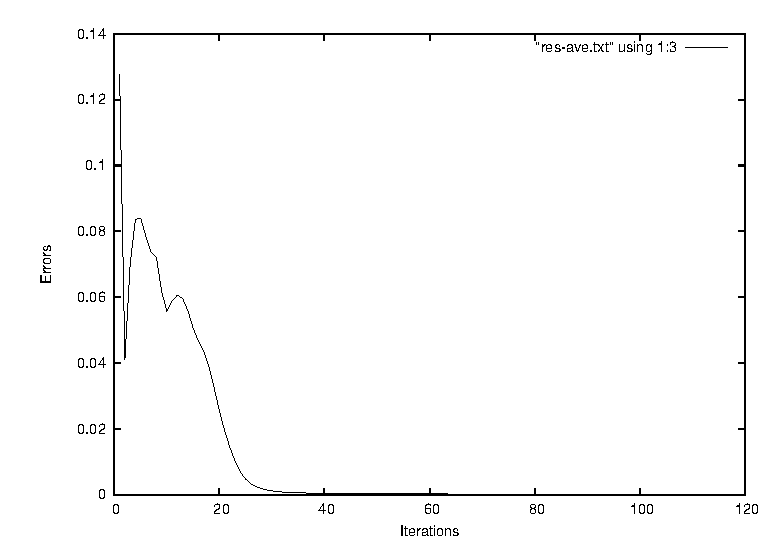
\includegraphics[width=10.0cm]{figs/sample2.eps}
  \caption{重みを更新する様子(平均値)}
  \label{fig:level2}
 \end{center}
\end{figure}


\subsubsection{考察}



\newpage

\section{Level3: 応用事例:文字認識問題への適用}
\subsection{課題説明}

最急降下法が苦手とする状況についてその理由を解説し,
検討した改善方法について解説する.

\subsubsection{原因}

「山(谷)」の数は一つにも関わらず最も勾配の高い方向に移動するため,一直線に谷には向かわずジグザグ移動してしまい,効率的ではない.

\subsubsection{改善方法}

・複数の初期値から探索を行いより短い探索で解にたどり着ける初期値を探す.\\
最適解の近傍に初期値を設定することができれば,余計な探索を減らすことができると考えた.
最適解のx軸方向の直線上に近い場所に初期値を設定することができれば,一直線に谷に向かうことも可能となる.\\\\


・また収束速度を安定させる手法として,前回得られた勾配ベクトルと今回得られた勾配ベクトルの符号の変化によって刻み幅の調整をする方法がある.符号が反転したときに刻み幅を小さくし,符号が等しいときに刻み幅を大きくすることで安定して収束する.





 %課題説明
\subsection{Level3.1: パラメータのチューニング}
\subsubsection{最適なパラメータを探すためのアプローチ}
指定された条件下において学習が効率良く行われるパラメータの組み合わせを探
すため、**して**することでパラメータを調整した。

(補足:全パターンを調べても良いし、いくつかのパターンを調べても良いが、
どのような方法で調整したら良いかを考えよう。その上で、自分たちがどのよ
うに取り組んだのか(=アプローチ)を説明しよう。)

\subsubsection{実行結果}

(補足:ボーナスポイントの確認がありますので、シード値10パターンで試した際の収
束に要した学習回数と、その平均回数が分かるように明示してください。)
\begin{table}[htb]
 \begin{center}
  \caption{階層型NNによる文字認識問題の学習に要した回数}
  \label{table:level3}
  \begin{tabular}[htb]{r|l} \hline
   シード値 & 収束した回数 \\ \hline \hline
   100 & hoge \\ \hline
   200 & hoge \\ \hline
   300 & hoge \\ \hline
   400 & hoge \\ \hline
   500 & hoge \\ \hline
   600 & hoge \\ \hline
   700 & hoge \\ \hline
   800 & hoge \\ \hline
   900 & hoge \\ \hline
   1000 & hoge \\ \hline \hline
   10試行の平均値 & hoge \\ \hline
  \end{tabular}
 \end{center}
\end{table}

\begin{figure}[h]
 \begin{center}
  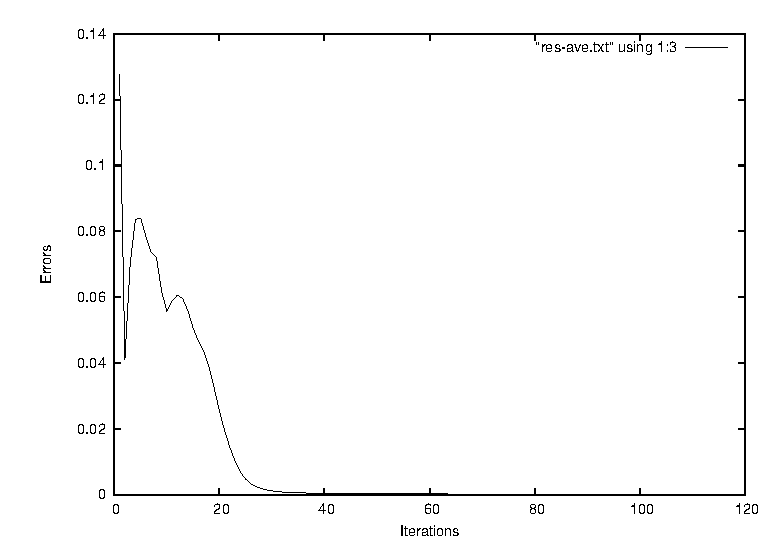
\includegraphics[width=10.0cm]{figs/sample2.eps}
  \caption{重みを更新する様子(平均値)}
  \label{fig:level2}
 \end{center}
\end{figure}


\subsubsection{考察}



\subsection{Level3.2: パラメータと収束能力の関連性について}
\subsubsection{関係性を確認するためのアプローチ}
HIDDENを固定してのETAの変更、ALPHAの変更を行っていき、値の変動を見て法則を確認する。

\subsubsection{結果}
ETAの変更による値の変化\\\\
HIDDEN : 30\\
ETA        : 0.5\\
ALPHA   : 0.72\\\\

指定シード値10パターンによる平均値 : 236\\

\\\\
HIDDEN : 30\\
ETA        : 0.6\\
ALPHA   : 0.72\\\\

指定シード値10パターンによる平均値 : 216.9\\

\\\\
HIDDEN : 30\\
ETA        : 0.7\\
ALPHA   : 0.72\\\\

指定シード値10パターンによる平均値 : 187\\


\\\\

~中略~\\\\

HIDDEN : 30\\
ETA        : 1.3\\
ALPHA   : 0.72\\\\

指定シード値10パターンによる平均値 : 108\\


\\\\
HIDDEN : 30\\
ETA        : 1.4\\
ALPHA   : 0.72\\\\

指定シード値10パターンによる平均値 : 129.5\\


\\\\
ALPHAの変更\\\\
HIDDEN : 30\\
ETA        : 1.3\\
ALPHA   : 0.73\\\\

指定シード値10パターンによる平均値 : 109.4\\


\\\\
HIDDEN : 30\\
ETA        : 1.3\\
ALPHA   : 0.71\\\\

指定シード値10パターンによる平均値 : 113.3\\


\\\\
HIDDENとETAの関係について\\\\
HIDDEN : 31\\
ETA        : 1.3\\
ALPHA   : 0.72\\\\

指定シード値10パターンによる平均値 : 93.1\\


\\\\
HIDDEN : 31\\
ETA        : 1.4\\
ALPHA   : 0.72\\\\

指定シード値10パターンによる平均値 : 105.1\\


\\\\
HIDDEN : 31\\
ETA        : 1.2\\
ALPHA   : 0.72\\\\

指定シード値10パターンによる平均値 : 92\\


\\\\
HIDDEN : 31\\
ETA        : 1.1\\
ALPHA   : 0.72\\\\

指定シード値10パターンによる平均値 : 88.1\\


\\\\
HIDDEN : 31\\
ETA        : 1.0\\
ALPHA   : 0.72\\\\

指定シード値10パターンによる平均値 : 99.1\\
\\\\

\subsubsection{考察}
上記実行結果を総合して考えた結果\\
HIDDENが大きくなると、早く収束する点でのETAの値はある一定まで小さくなり、HIDDENが小さくなると、早く収束する点でのETAの値は一定まで大きくなる、という関係があるように思えた。





\subsection{Level3.3: 任意の評価用データを用いた評価}
\subsubsection{アプローチ}
(仮説1)\\
学習時のデータ(教師データ)との違いが少ない程認識率が高く、
逆に教師データとの違いが多い程認識率が低くなるとの仮定の下、
如何に示す評価データを用意した。
\begin{itemize}
	\item a\_deter1.txt
	\item a\_deter2.txt
	\item a\_deter3.txt
	\item a\_deter4.txt
	\item a\_deter5.txt
	\item a\_deter6.txt
\end{itemize}

 (仮説2) \\
 学習時のデータ(教師データ)との違いが多い程認識率が高く、
 逆に教師データとの違いが少ない程認識率が低くなるとの仮定の下、
 評価データは仮説1と同様のものを用いる。

(仮説3)\\
学習データの一部分だけの場合,一部分が似ているものの認証率が高いという仮定の下,
「あ」のデータを上下左右の半分だけのデータを用意した.また他の文字の左半分だけのデータも用意した.
\begin{itemize}
	\item a\_up.txt
	\item a\_down.txt
	\item a\_left.txt
	\item a\_half.txt 
	\item ka\_half.txt
	\item sa\_half.txt
	\item ta\_half.txt
	\item na\_half.txt
	\item ha\_half.txt
	\item ma\_half.txt
	\item ya\_half.txt
	\item ra\_half.txt
	\item wa\_half.txt
\end{itemize}


\subsubsection{結果}
\begin{figure}[h]
 \begin{center}
  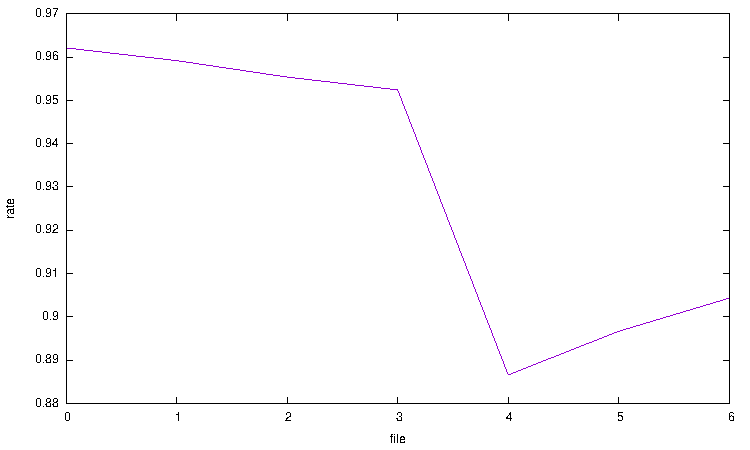
\includegraphics[width=10.0cm]{figs/level3/deter.pdf}
  \caption{仮説1:認証率(rate)と違い}
  \label{fig:level3_3_1}
 \end{center}
\end{figure}
上記のX軸は,0が学習データと同じデータ,1以降はa\_deter.txtの番号となっている.またこの番号が上がるにつれて,元データよりデータを劣化(1-$>$0)にしている.

\begin{figure}[h]
 \begin{center}
  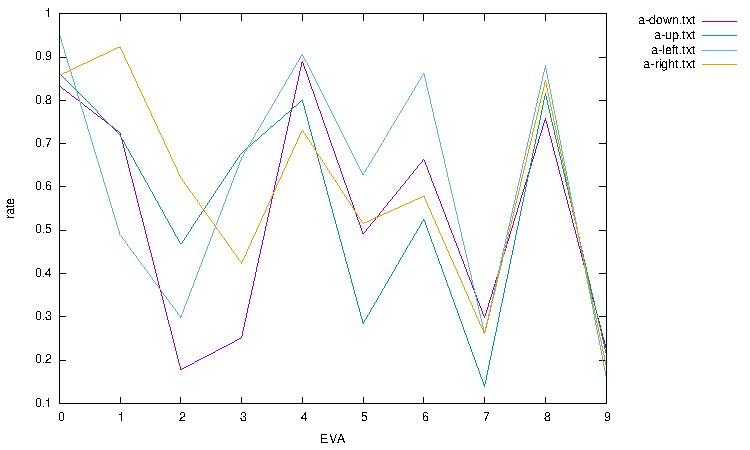
\includegraphics[width=10.0cm]{figs/level3/adata.pdf}
  \caption{仮説3:「あ」のデータ}
  \label{fig:level3_3_2}
 \end{center}
\end{figure}

\begin{figure}[h]
 \begin{center}
  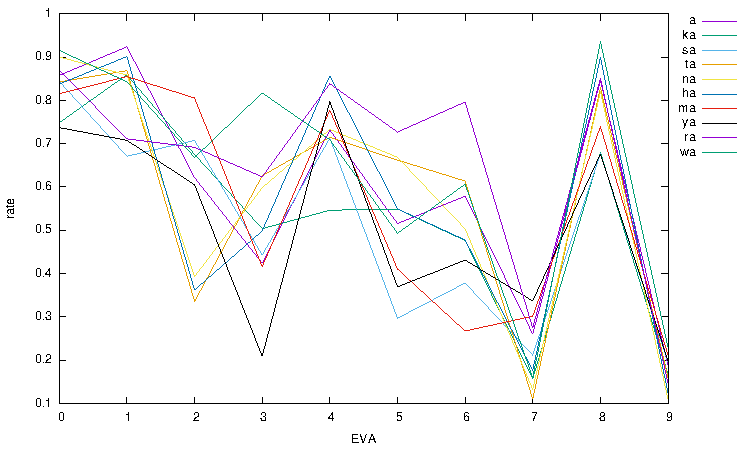
\includegraphics[width=10.0cm]{figs/level3/mozi.pdf}
  \caption{仮説3:学習データすべての半分}
  \label{fig:level3_3_3}
 \end{center}
\end{figure}

\subsubsection{考察}
結果として
\begin{itemize}
	\item 仮説1,2: 違いが増えるほど認証率は低くなるが,ほとんどデータを劣化させた場合少し高くなる.
	\item 仮説3: 「あ」のデータを移動させた場合,「あ」としての認証率が高く,他にも「な」や「ら」,「か」などの文字としての認証率も高かった.
	\item 仮説3: 学習データ全ての文字を半分にしてみた場合,「あ」,「か」,「な」,「ら」の認証率が高かった.
\end{itemize}
というデータを得た.\\
図\ref{fig:level3_3_1}のデータの中で,ほとんどデータを劣化させたa\_deter5.txtとa\_deter6.txtの認証率が若干高くなったのは,ほとんどデータが少なく判断できなかったことで全体的に認証率が上がったのではないかと推測する.\\
図\ref{fig:level3_3_2},\ref{fig:level3_3_3}より,似た部分の多い「あ」,「か」,「な」,「ら」の4つの認証率が高いことがわかった.\\
よって,仮説1と3が正しいという結果になった.

\subsection{Level3.4: 認識率を高める工夫}
\subsubsection{対象とする問題点}
入力されたデータが想定していた入力と比べてサイズが異なったり、位置がずれている等、文字の一部が欠けている以外にも多様な要因によるデータ(情報)の劣化が考えられる。認識率を高めるにはどのような点を工夫すれば良いか?どのような方法でも構わないので、検討せよ。

\subsubsection{改善方法の提案}
認識率を高めるために改善すべき方法として,学習データの数を増やすということがあげられる.

\subsubsection{考察}
今回の実験では,学習サンプルデータがそれぞれ1種類ずつしかなかった.
そのため,いろいろなパターンの文字の形を学習させる際に少々学習に手間取ったように見える.
この問題を解決するための方法として学習データの増加を行うという方法がある.

人の脳をモデルとしているのならば,人が行うような学習をさせれば良い.
いろいろなデータを蓄えておいて,それを元に分析を行うことはごく自然なことである.
一つの事象にとらわれることなく学習を行うために,データの増加は必要だと考えた.
1つの文字に対して複数のパターンを用意し,それに基づいて学習をさせれば,与えたデータをより細かく学習させることができるだろう.

この方法の実装を今回試みたが,ニューロンの多層化が必要になり,単純なコード変更では期待していた結果が得られなかった.\\

また,別の方法として,データを複数のパターンを用意して,それに共通する部分や同じような形をプログラム上で記憶させておけば,さらに学習パターンは広がるはずだ.

\newpage
\section{その他: 実験の内容・進め方に関するコメント等}
(補足:
今後の為に参考にしたいので、情報工学実験2・探索アルゴリズム1,2で扱った
内容、実験の進め方等について意見があれば書いてください(当然、どのような
意見であってもレポートの評価を下げる事はしません。)。「授業評価アンケー
ト」の際に書いてもらっても構いません。)


\vspace{+1.0cm}
(補足:参考文献は thebibliography 環境を使って列挙し、
本文中で適切な箇所で引用するようにしましょう。
例えば下記文献は、アブストラクト中で引用しています)
\begin{thebibliography}{99}
\bibitem{info2-search2}
情報工学実験2: 探索アルゴリズムその2(當間)\\
\verb|http://www.eva.ie.u-ryukyu.ac.jp/~tnal/2011/info2/search2/|
\end{thebibliography}

\end{document}
